\section{HEC-RAS Unsteady}
%%%%%%%%%%%%%%%%%%%%%%%%%%%
what is HEC-RAS?
what is unsteady?
\subsection{Installation Verification}
The software install was demonstrated in Lesson 3.
Here we just want to check the install.
Easiest way is to start the program and run one of the example

\begin{figure}[h!] %  figure placement: here, top, bottom, or page
   \centering
   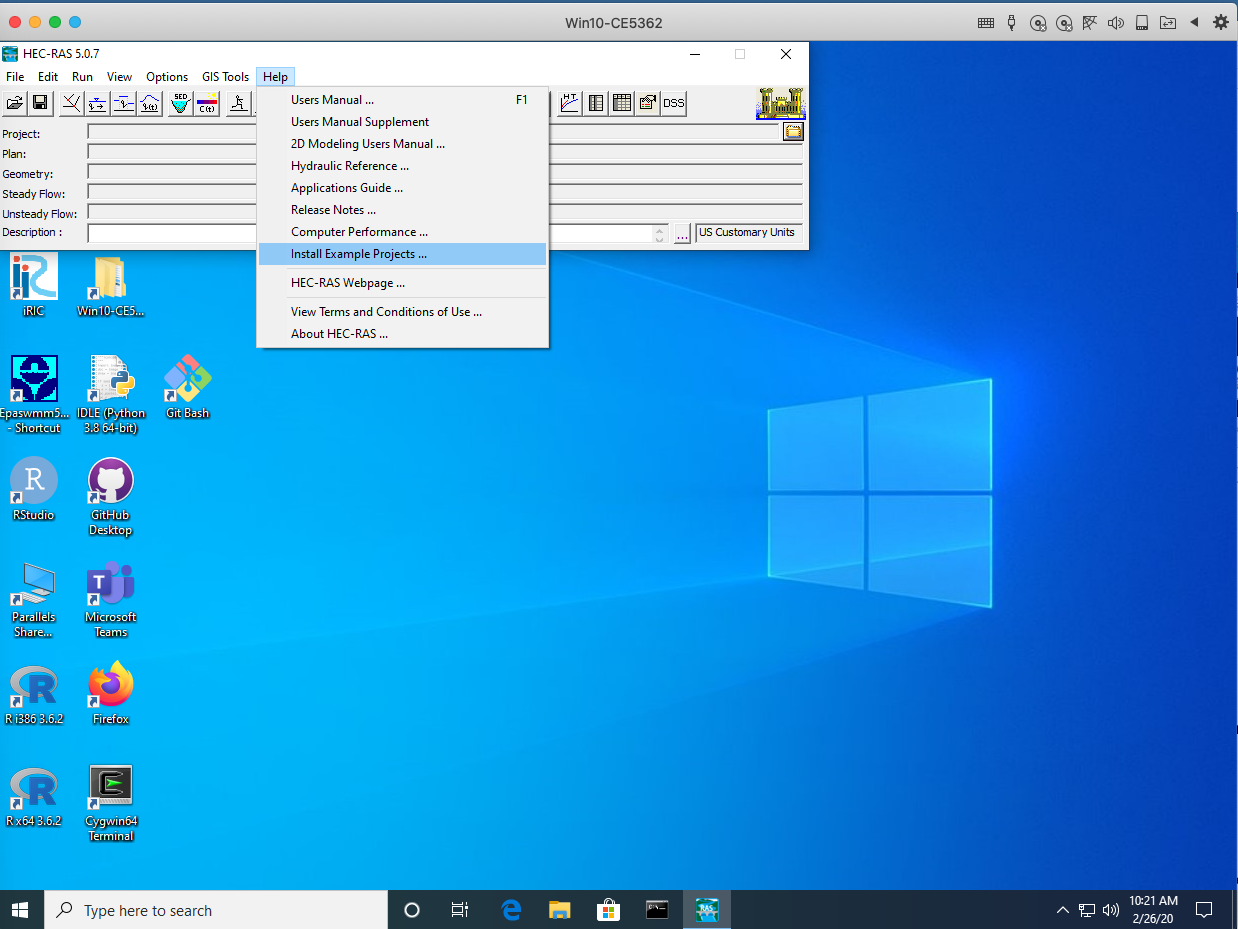
\includegraphics[width=4in]{help-install-examples.png} 
   \caption{Start from desktop, HELP/INSTALL EXAMPLES from navigation menu.}
   \label{fig:help-install-examples}
\end{figure}



\begin{figure}[h!] %  figure placement: here, top, bottom, or page
   \centering
   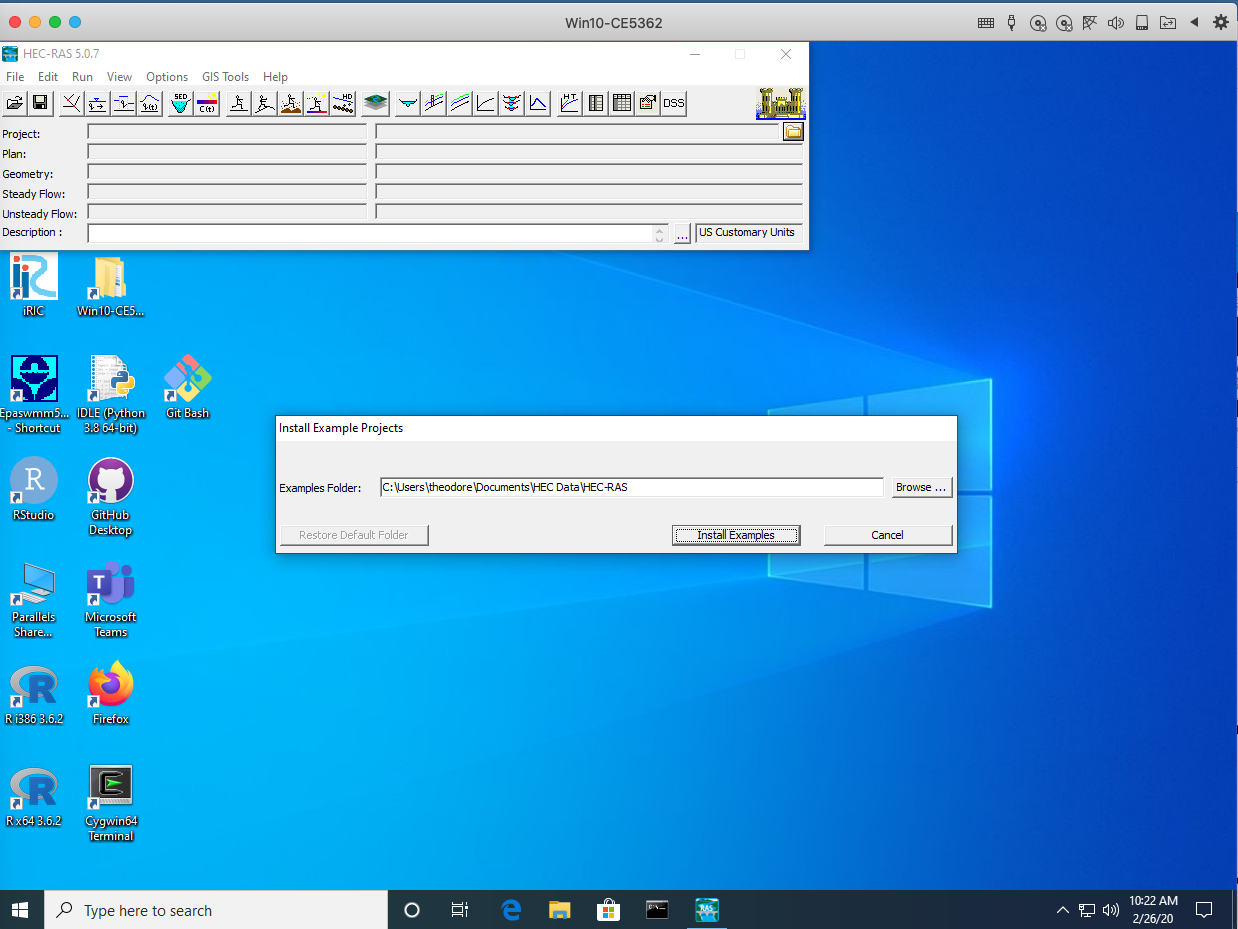
\includegraphics[width=4in]{select-install-examples.png} 
   \caption{Select the path to the examples, and instruct the program to install its examples}
   \label{fig:select-install-examples}
\end{figure}



\begin{figure}[h!] %  figure placement: here, top, bottom, or page
   \centering
   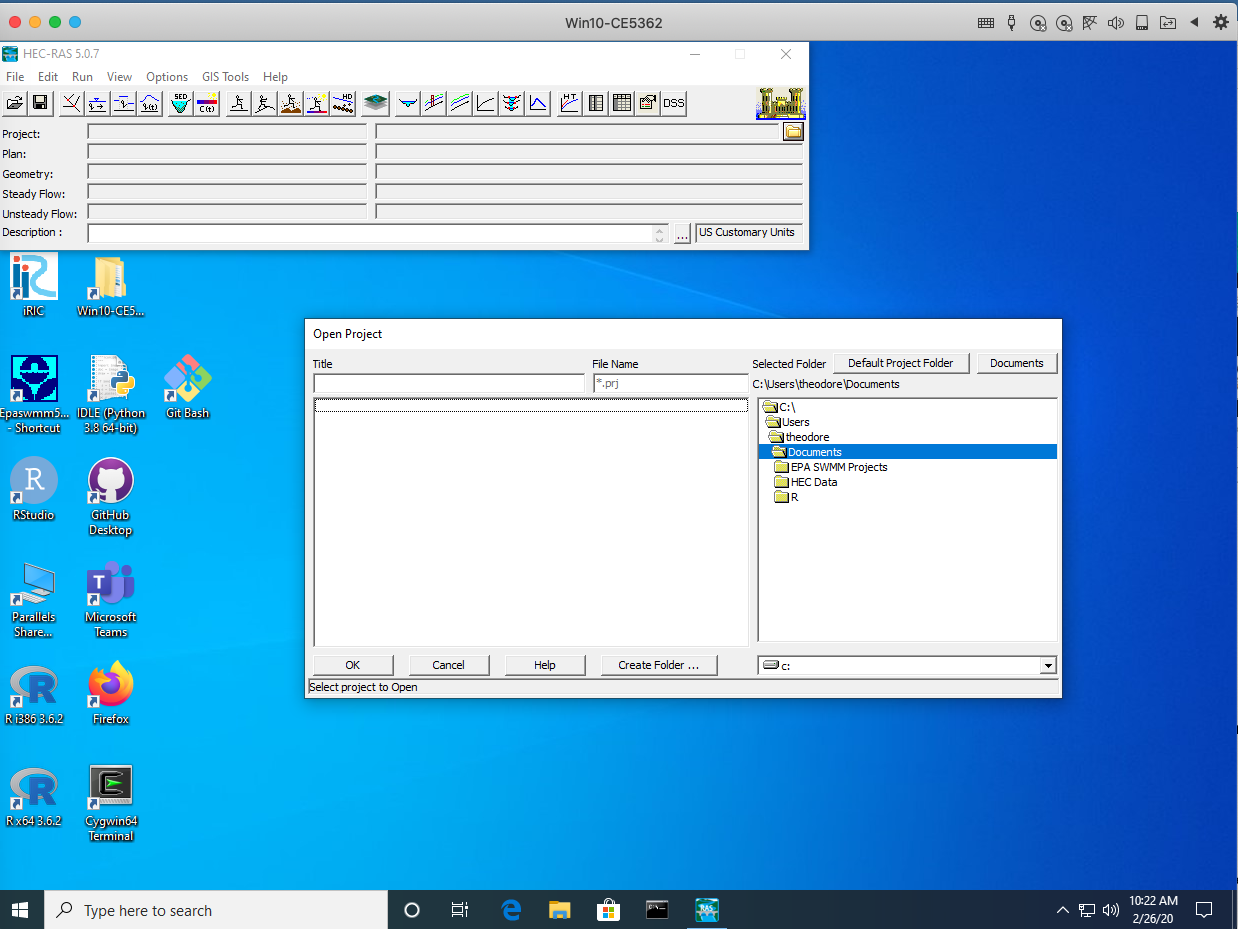
\includegraphics[width=4in]{file-open-projects.png} 
   \caption{Select FILE/OPEN PROJECTS}
   \label{fig:file-open-projects}
\end{figure}


\begin{figure}[h!] %  figure placement: here, top, bottom, or page
   \centering
   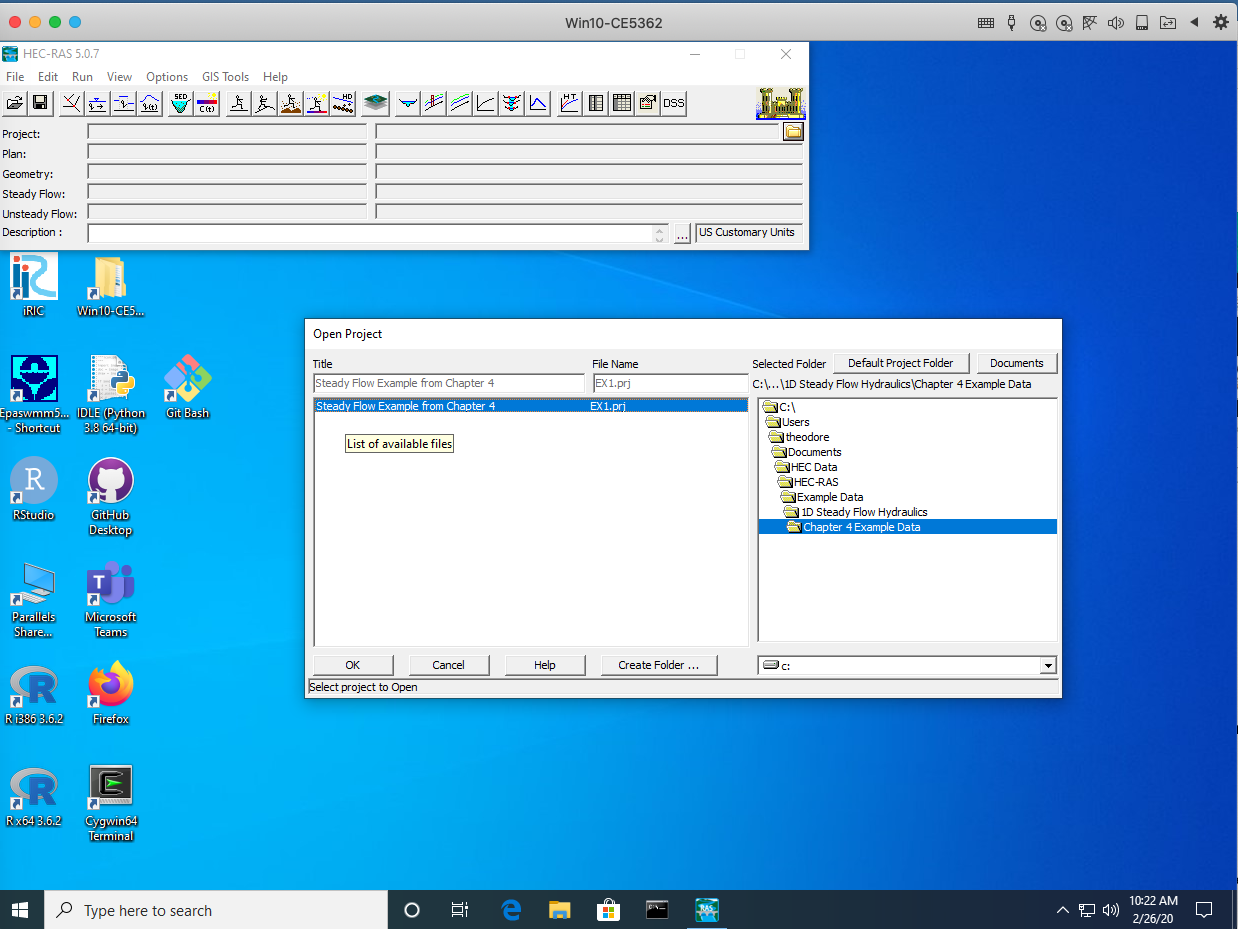
\includegraphics[width=4in]{navigate-projects-select.png} 
   \caption{Navigate to examples and select one, here I choose steady Chapter 4 Example}
   \label{fig:navigate-projects-select}
\end{figure}

\clearpage

\begin{figure}[h!] %  figure placement: here, top, bottom, or page
   \centering
   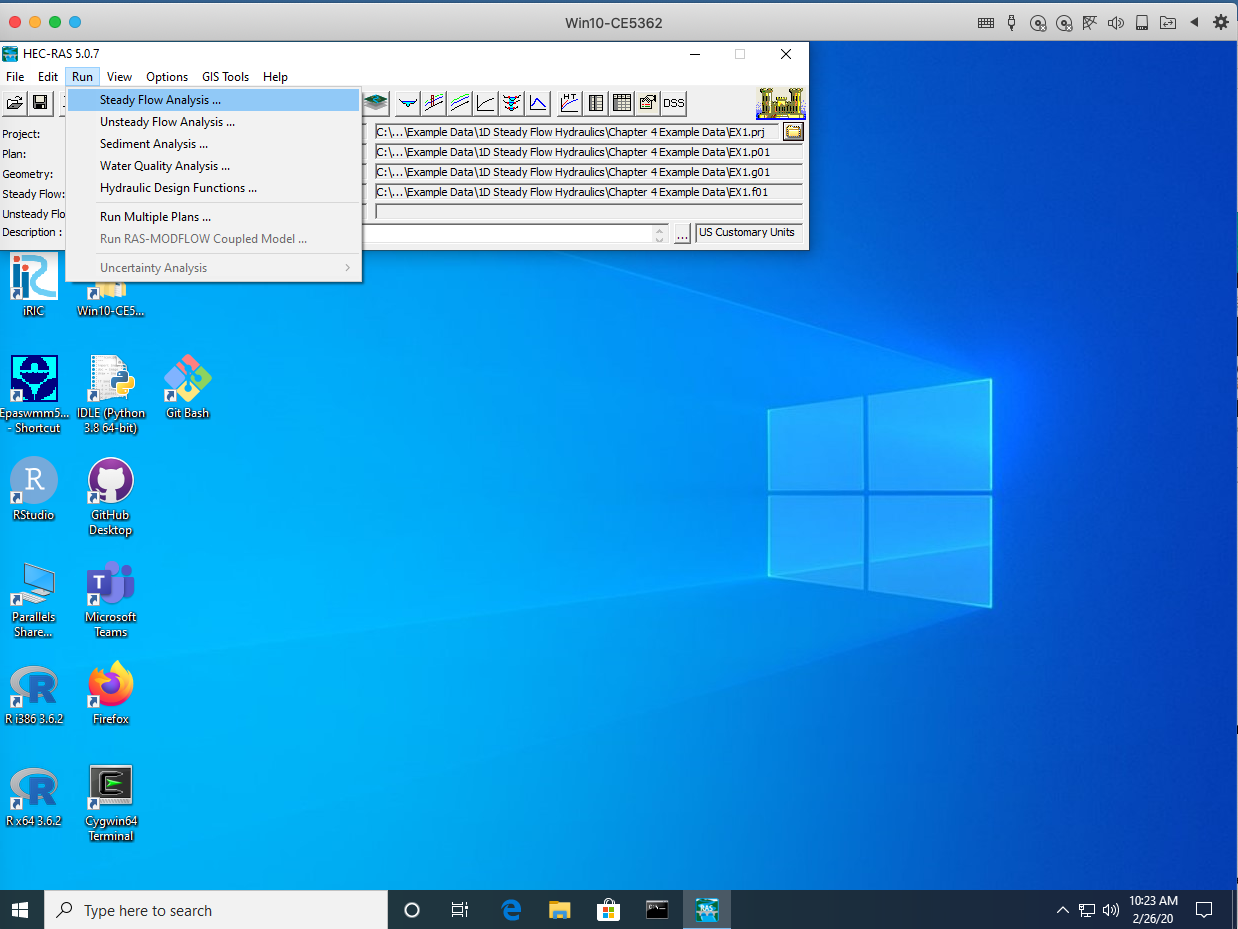
\includegraphics[width=4in]{run-steady-analysis.png} 
   \caption{Navigate to RUN/STEADY ANALYSIS; and then run the analysis }
   \label{fig:run-steady-analysis}
\end{figure}



\begin{figure}[h!] %  figure placement: here, top, bottom, or page
   \centering
   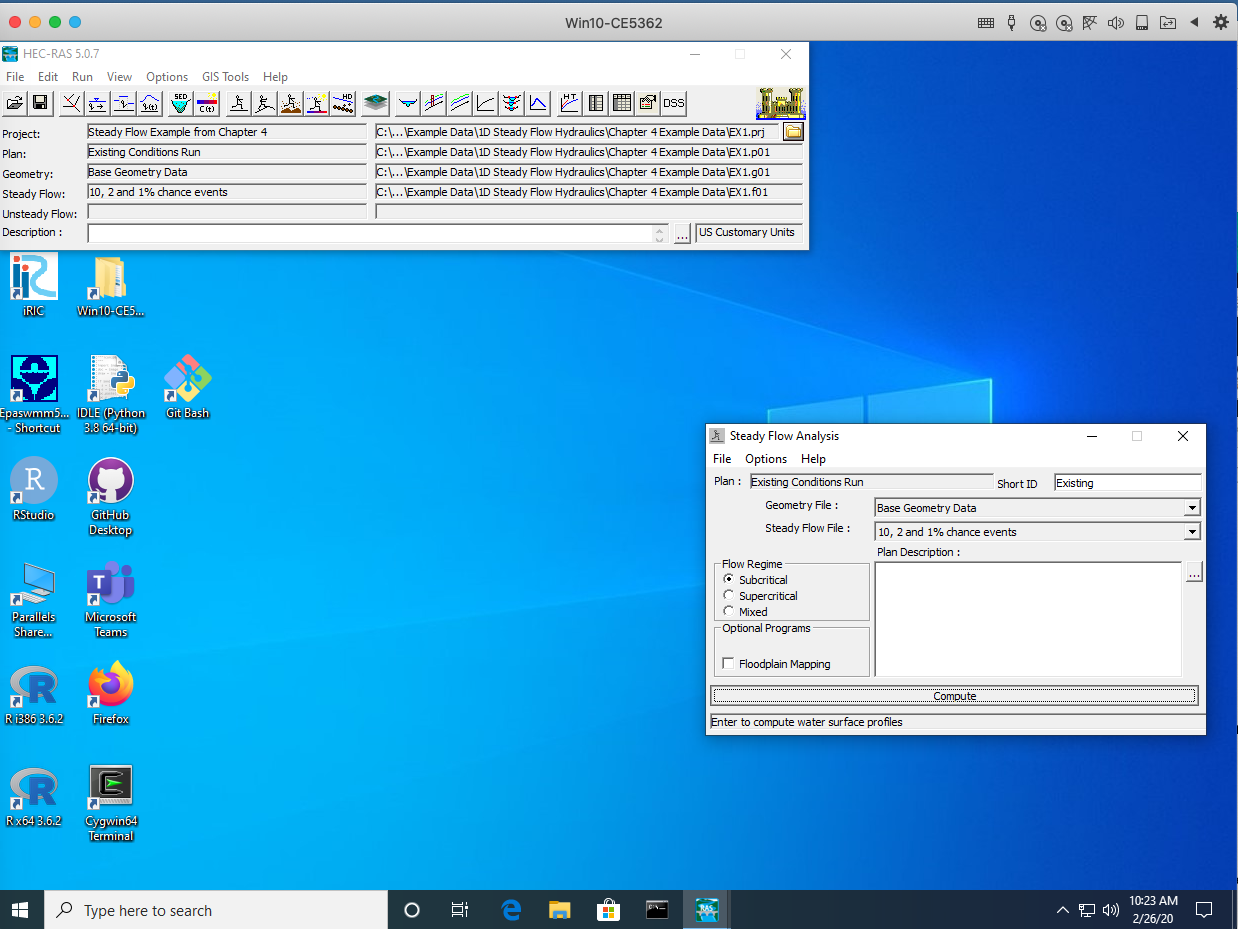
\includegraphics[width=4in]{select-plan-compute.png} 
   \caption{Select COMPUTE, let the program run}
   \label{fig:select-plan-compute}
\end{figure}

\clearpage

\begin{figure}[h!] %  figure placement: here, top, bottom, or page
   \centering
   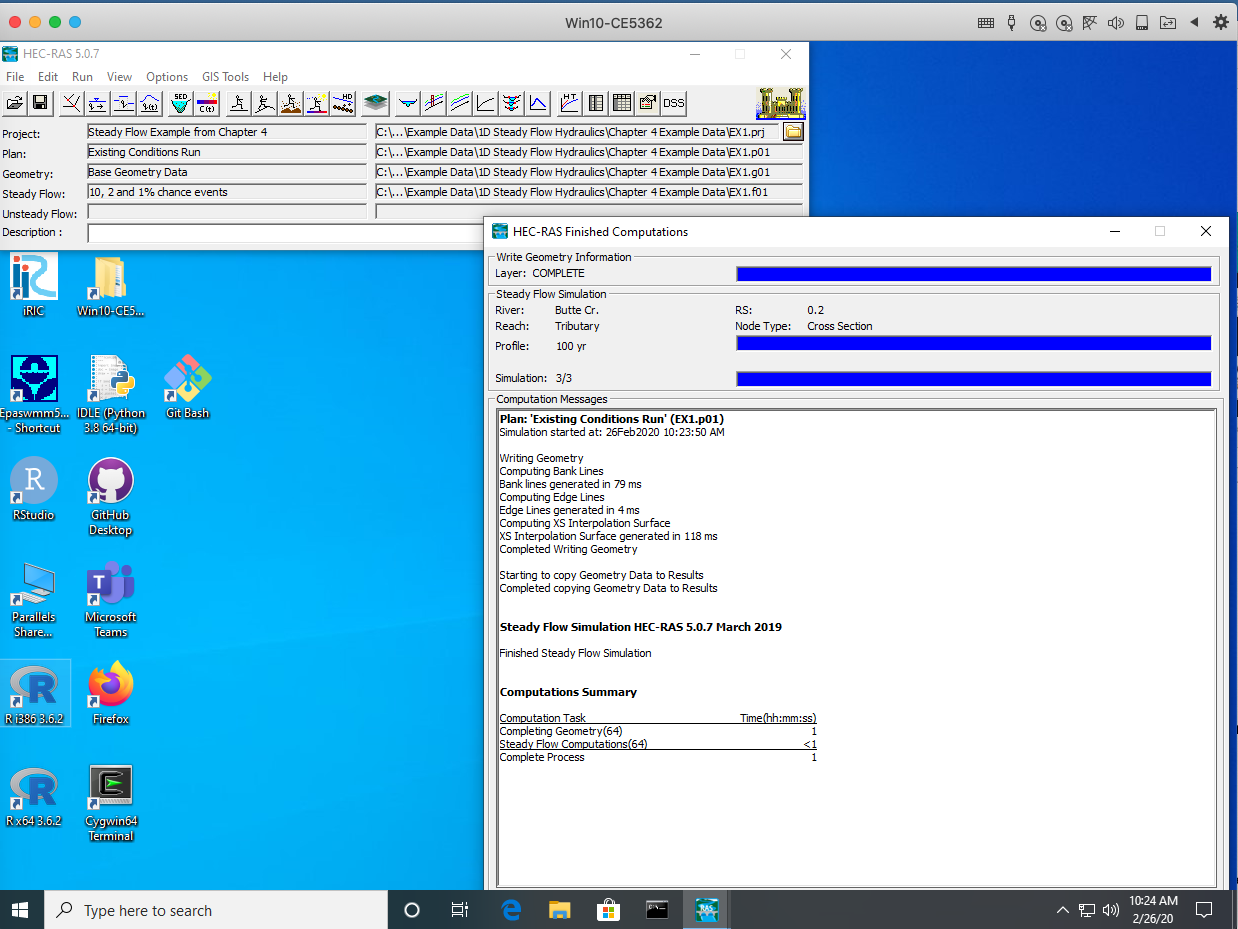
\includegraphics[width=4in]{hecras-done.png} 
   \caption{Expected completion appearance; thus we conclude the program is correctly installed and paths are established.}
   \label{fig:hecras-done}
\end{figure}

\subsection{Interface Tour}

\clearpage
\subsection{Examples}
\subsubsection{Example 1.A -- Rectangular Channel using HEC-RAS Steady}
Figure \ref{fig:example1} is a backwater curve\footnote{Page 85. Koutitas, C.G. (1983). Elements of Computational Hydraulics. Pentech Press, London 138p. ISBN 0-7273-0503-4 } for a rectangular channel with discharge over a weir (on the right hand side --- not depicted).  The channel width is 5 meters, bottom slope $0.001$, Manning's $n=0.02$ and discharge $Q=55.4 \frac{m^3}{sec}$.  
Use HEC-RAS steady to reproduce the backwater curve on 1000- meter spacing

\begin{figure}[h!] %  figure placement: here, top, bottom, or page
   \centering
   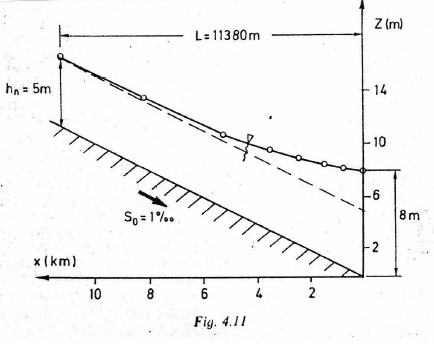
\includegraphics[height=2.5in]{bw_curve1.jpg} 
   \caption{Example backwater curve} 
   \label{fig:example1}
\end{figure}


\subsubsection{Example 1.B -- Rectangular Channel using HEC-RAS Unsteady}
The backwater curve situation for a rectangular channel with discharge over a weir is repeated, but an unsteady input is implemented (a couple step changes in flow) to illustrate how to enter transient boundary conditions.

\subsubsection{Example 2.A -- Non-prisimatic channel using HEC-RAS Steady}
A plan view of a  channel of variable width as shown in Figure \ref{fig:NonPrismaticExample}.\\

\begin{figure}[h!] %  figure placement: here, top, bottom, or page
   \centering
   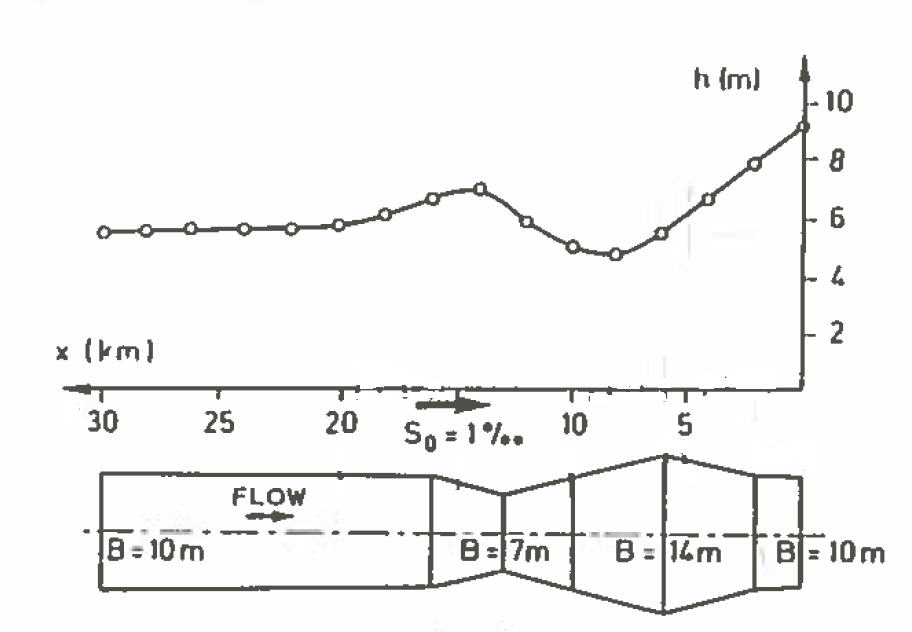
\includegraphics[width=2.5in]{NonPrismaticExample} 
   \caption{Non-Prismatic Rectangular Channel}
   \label{fig:NonPrismaticExample}
\end{figure}

The channel conveys $Q=100~m^3/sec$, with a bottom slope of $0.001$ and average Manning's $n$ value of $0.033$.  
A backwater curve is caused by a weir at the downstream end (to the right in the figure) by a 7 meter tall weir.
Flow depth over the weir is at critical depth $h_c = 2.17$ meters.    

Use HEC-RAS steady to reproduce the backwater curve on 1000- meter spacing

\subsubsection{Example 2.B -- Non-prisimatic channel using HEC-RAS Unsteady}
The backwater curve situation for a non-prisimatic rectangular channel with discharge over a weir is repeated, but an unsteady input is implemented (a couple step changes in flow) to illustrate how to enter transient boundary conditions.

\subsubsection{Example 3 -- Sudden Gate Closing in an Aqueduct Channel}
Flow in a 1000-m long trapezoidal channel with a bottom width of 20-m, side slope of 2H:1V, longitudinal slope $S_0$=0.0001, and Manning's resistance n=0.013. 
Initial discharge in the channel is 110 m3/s and initial flow depth is 3.069 m.
Simulate the flow and depth at every 100-m station when a downstream gate is closed at t=0. 
Produce a graph of depth and velocity versus location for t=0, 60, 360 seconds.\footnote{Example 12-1, Page 623. Roberson, J A., Cassidy, J.J., and Chaudhry, M. H. (1988). Hydraulic Engineering. Houghton Mifflin Co., Boston, 662p. }

\subsubsection{Example 4 -- Flood Hydrograph in Horizontal Channel}
The initial depth in a horizontal channel of rectangular cross section is 1 meter. 
The channel is 29 kilometers long and ends with a non-reflection boundary condition.
\newpage
\begin{figure}[h!] %  figure placement: here, top, bottom, or page
   \centering
   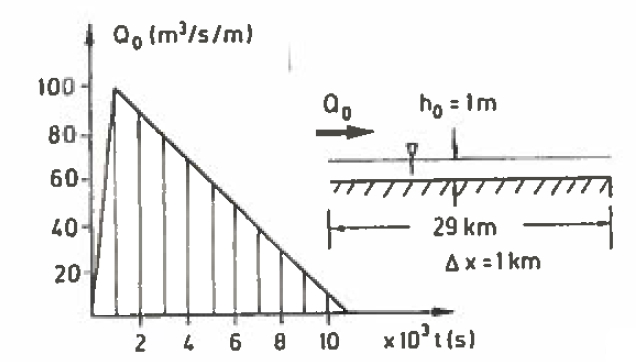
\includegraphics[width=4.25in]{upstreamHydro.jpg} 
   \caption{Upstream hydrograph for example}
   \label{fig:upstreamHydro}
\end{figure}

The initial discharge in the channel is 0 cubic meters per second. 
The upstream input hydrograph is shown in Figure \ref{fig:upstreamHydro}.
The manning friction factor is $n=1/40$.
Simulate the water surface elevation over time in the channel.\footnote{Example 4.1, Page 70. Koutitas, C.G. (1983). Elements of Computational Hydraulics. Pentech Press, London 138p. ISBN 0-7273-0503-4 }


\subsubsection{Example 5 -- Long waves in a Tidal-Influenced Channel}


\subsection{Appendix}
